\section{基本要求二：SysY 程序的 LLVM IR 与 RISC-V 等价实现及验证}
\label{sec:sysy}
\subsection{SysY 示例程序设计与语言特性覆盖}
\label{sec:sysy-coverage}
本实验设计两个互补的 SysY 示例，以整数控制逻辑和浮点数据处理分别检验语言特性的实现。先确定源程序的计算语义、有效输入域与独立预期，再分别分析手写 LLVM IR 和 RISC-V 汇编，最后通过运行库集成、目标程序构建与运行测试检查语义一致性。

\subsubsection{示例程序设计与语言特性覆盖}
\label{sec:sysy-example-design}
\texttt{control\_matrix} 检验整数运算、赋值与初始化、条件分支、循环、\texttt{break/continue}、短路副作用、二维数组、函数调用、作用域及有符号除余；\texttt{float\_stats} 检验单精度浮点运算、一维浮点数组、函数调用、整数与浮点混合参数以及类型转换。两个程序各有 SysY 源程序，以及独立手写的 \texttt{.ll/.S} 等价实现，便于对照同一源语义在不同抽象层次中的表达。

表\ref{tab:coverage}将课程要求逐项对应到两个源程序中的构造，并列出 IR 或汇编实现机制。表中的位置以函数、变量或表达式标识，便于将语言特性与后续分析联系起来。
\Needspace{14\baselineskip}
\begingroup
\small
\setlength{\tabcolsep}{5pt}
\begin{longtable}{L{2.35cm}L{6.35cm}L{5.6cm}}
\caption{课程语言特性要求与 SysY 示例覆盖位置}
\label{tab:coverage}\\
\toprule\rowcolor{tableHead}课程要求 & 本实验源码位置 & 对应机制与验证 \\
\midrule
\endfirsthead
\toprule\rowcolor{tableHead}课程要求 & 本实验源码位置 & 对应机制与验证 \\
\midrule
\endhead
\bottomrule
\endfoot
\texttt{int/float} 与变量声明 & \texttt{control\_matrix} 的 \texttt{n/i/sum}；\texttt{float\_stats} 的 \texttt{scale/result} & \texttt{i32/float} 类型；整数与单精度浮点分别运算。\\
常量与初始化 & \texttt{COLS=3}、\texttt{SHIFT=0.25}；整数二维数组与浮点一维数组初值 & \texttt{COLS} 用于行列索引计算，\texttt{SHIFT} 用于结果偏置；二维数组部分初始化补零。\\
数值运算 \texttt{+,-,*} & \texttt{tick} 的一元 \texttt{+x}；\texttt{fold} 的 \texttt{n-1}、\texttt{sum+v*i}；\texttt{affine} 的乘加 & 一元加保持值；\texttt{add/sub/mul} 与 \texttt{fmul/fadd}。\\
数值运算 \texttt{/,\%} & \texttt{cell} 调用参数 \texttt{i/COLS,i\%COLS}；整数输出中的除余；\texttt{normalized} 的浮点除法 & \texttt{sdiv/srem} 与 \texttt{divw/remw}；\texttt{fdiv/fdiv.s}。\\
关系运算 & 整数 \texttt{fold/main} 覆盖 \texttt{<=,<,>,==,!=}；\texttt{sum\_positive} 的整数循环条件使用 \texttt{>=}，浮点筛选使用 \texttt{v>0.0} & 整数 \texttt{icmp}、浮点 \texttt{fcmp} 与条件分支。\\
\texttt{\&\&,||,!} & 整数 \texttt{main} 中两条含 \texttt{tick} 的条件及 \texttt{if(!gate)} & 短路以控制流实现；全局 \texttt{calls} 记录副作用次数。\\
赋值 & \texttt{calls=calls+1}、\texttt{sum=sum+v*i} 与 \texttt{a[i]=getfloat()} & SSA 新值、全局/数组 \texttt{store}；汇编寄存器和内存更新。\\
\texttt{if/while} & \texttt{fold} 的循环与判断；\texttt{sum\_positive} 的正值筛选 & 条件基本块、回边与汇编 branch/label。\\
\texttt{return} & \texttt{tick/cell/fold/affine} 返回值；\texttt{separator} 的无值返回 & LLVM \texttt{ret}；整数/浮点返回使用 \texttt{a0/fa0}。\\
\makecell[l]{\texttt{break}\\\texttt{continue}} & \texttt{fold} 中零值跳过与 stop 提前终止 & \texttt{body}$\to$\texttt{step} 与 \texttt{check.break}$\to$\texttt{exit}；phi 与回边。\\
函数定义与调用 & \texttt{cell/fold/tick}；无参 void 函数 \texttt{separator}；\texttt{affine/sum\_positive} & 带参返回函数与无参 void 函数；\texttt{call} 与 ABI 传参。\\
作用域 & 全局 \texttt{bias=7} 与整数 \texttt{main} 内层块的 \texttt{bias=3} & 名字遮蔽后分别贡献 7 与 3，全局变量值未被局部声明改变。\\
一维/二维数组 & 两个 \texttt{main} 中的 \texttt{float a[4]}、\texttt{int a[2][3]}；\texttt{cell(int a[][3],...)} & 浮点元素 GEP 与行指针 GEP；二维行跨度 12 字节。\\
浮点与混合调用 & \texttt{affine(float x,float scale,int offset)}、\texttt{sum\_positive} & 整数/浮点参数寄存器独立分配；binary32 舍入。\\
类型转换 & \texttt{affine} 将整数 offset 加入浮点乘积；\texttt{int truncated=result} & \texttt{sitofp/fcvt.s.w}；\texttt{fptosi/fcvt.w.s rtz} 向零截断。\\
输入输出与运行库 & \makecell[l]{\texttt{getint/getfloat}\\\texttt{putint/putfloat/putch}} & 静态链接 SysY 运行库，调用目标 glibc。\\
张量类型 & 未覆盖 & 课程材料未提供具体语法与语义定义。\\
\end{longtable}
\endgroup

\subsubsection{\texttt{control\_matrix}：整数运算与控制流}
\label{sec:sysy-integer-semantics}

该程序对更新后的二维整数数组进行带提前终止条件的加权求和，同时输出短路调用次数、条件分支标记和有符号除余结果。\texttt{cell} 按给定行、列返回数组元素；\texttt{fold} 将线性位置分别除以和取余 \texttt{COLS}，据此访问对应元素。

二维部分初始化 \texttt{\{\{1,2\},\{-3,4,5\}\}} 产生 $[1,2,0,-3,4,5]$。输入是 \texttt{n}、\texttt{stop}、\texttt{gate}、\texttt{divisor} 和六个增量；更新后元素记为 $a_i$。\texttt{fold} 检查前 $n$ 个位置，先递增索引，遇 0 执行 continue，遇非零 stop 执行 break，其余贡献 $(i+1)a_i$；第一项输出再加全局 7 与局部 3。因此 stop=0 不会把零元素当作停止点。

其余输出为 \texttt{calls,tag,q,r}。gate=0 时 \texttt{\&\&} 的 RHS 和 \texttt{||} 已为真的左侧之后的 RHS 均跳过，故 \texttt{calls=0,tag=6}；gate 非零且首元素正、末元素负时，两次 tick 均执行，得到 \texttt{calls=2,tag=3}。SysY 将 \texttt{Exp} 与 \texttt{Cond} 分开，括号基本表达式只包围 \texttt{Exp}；源码中的布尔条件依赖 \texttt{\&\&} 高于 \texttt{||} 的优先级组织，符合这一文法约束。

\texttt{calls} 记录 \texttt{tick} 对全局状态的修改次数，\texttt{tag} 记录三条条件语句的分支结果；\texttt{q,r} 分别是更新后 \texttt{a[0][1]} 除以 \texttt{divisor} 的商与余数。内层块中的 \texttt{bias=3} 遮蔽全局名字，只将 3 赋给 \texttt{local}，不改变全局 \texttt{bias=7}，两者在第一项输出中分别贡献偏置。

有效域为 $0\le n\le6$、增量 $[-30,30]$、stop $[-40,40]$、gate $[-2,2]$，divisor 为 $[-7,7]$ 内非零数，保证无越界、溢出、除零及 \texttt{INT\_MIN/-1}。oracle 直接计算首个非零 stop 之前的加权前缀和；商以绝对值整除后补符号，余数用 $r=a-qd$，避免误用 Python 对负数向下取整的语义。

\subsubsection{\texttt{float\_stats}：浮点运算与函数调用}
\label{sec:sysy-float-semantics}
\texttt{float\_stats} 对一维数组元素进行仿射变换，筛选正值并累加，再输出带偏置的结果及其两种派生值。程序输入为整数 \texttt{n}、单精度 \texttt{scale} 和 \texttt{n} 个浮点元素。\texttt{float a[4]} 初值为 $[1.0,-2.0,0.5,0.0]$，输入覆盖前 \texttt{n} 项，未参与计算的其余元素不影响结果。

\texttt{affine(float x,float scale,int offset)} 计算 \texttt{x*scale+offset}，其中整数 \texttt{offset} 转为浮点后参与加法。\texttt{sum\_positive} 从 \texttt{i=0,sum=0.0} 开始，在整数条件 \texttt{n>=i+1} 成立时调用 \texttt{affine(a[i],scale,i)}；仅当返回值 \texttt{v>0.0} 时将其加入累计和，然后递增索引。该设计同时覆盖浮点函数返回值、混合类型参数、正值筛选和有序累加。

\Needspace{10\baselineskip}
源程序的预期必须包含单精度舍入，而非仅按实数计算最终公式。记 $\operatorname{fl}_{32}$ 为独立数值 oracle 使用的 binary32 舍入，输入的 \texttt{a} 和 \texttt{scale} 已转换为 binary32。第 $i$ 项及累计状态为
\begin{equation}
\begin{aligned}
p_i&=\operatorname{fl}_{32}(a_i\,scale),&
v_i&=\operatorname{fl}_{32}\bigl(p_i+\operatorname{fl}_{32}(i)\bigr),\\
S_0&=0,&
S_{i+1}&=
\begin{cases}
\operatorname{fl}_{32}(S_i+v_i),&v_i>0,\\
S_i,&v_i\le0.
\end{cases}
\end{aligned}
\label{eq:sysy-float-oracle}
\end{equation}
乘法、仿射加法与每次累加分别舍入，不将乘加合并为一次运算。随后 \texttt{result} 为累计和加 0.25 后的 binary32 结果，\texttt{truncated} 为 \texttt{result} 向零截断得到的整数；\texttt{normalized} 将同一 \texttt{result} 除以整数 $n+1$ 转换后的浮点值，并再次舍入。程序按 \texttt{result,truncated,normalized} 的顺序输出，以空格分隔、换行结束。这里的 \texttt{normalized} 分母为 \texttt{n+1}，分子包含正值筛选与偏置，表示程序定义的归一化结果。

有效域为 $0\le n\le4$、有限数、$|scale|\le8,|a_i|\le32$；oracle 每步舍入至 binary32，浮点误差要求 $|y-\widehat y|\le10^{-6}+2\times10^{-6}|\widehat y|$，整数精确比较，不扩展到 NaN/Inf、次正规数或越界转换。\texttt{tests/sysy\_oracle.py} 使用 \texttt{struct} 的单精度打包与解包构造独立预期，明确区分乘、加、筛选、累加、偏置、向零转换和除法的先后次序。上述计算定义及独立预期是后续分析两种底层实现的依据。

\subsection{LLVM IR 等价实现与关键语义映射}
\label{sec:sysy-ir}
LLVM IR 用类型化指令表达运算，用基本块和分支表达控制流，用 SSA 值及 phi 节点表达变量更新。数组和全局变量仍通过内存访问实现。等价实现要求保留源程序的求值顺序、数据布局和副作用。

\subsubsection{基本块与条件控制流}
\label{sec:sysy-ir-blocks}
SysY 的 \texttt{if} 与 \texttt{while} 条件对应 LLVM 的比较指令和 \texttt{br}。例如 \texttt{fold} 的 \texttt{icmp sle} 决定进入循环体还是退出；\texttt{tick} 对全局变量的赋值则由 \texttt{load/add/store} 表达。为同时观察循环路径与短路路径，图\ref{fig:llvm-fold-cfg}分别展示 \texttt{fold} 与 \texttt{main} 的控制流。

图\ref{fig:llvm-fold-cfg}根据手写 IR 的终结指令绘制：\texttt{fold} 有七个块、九条边，\texttt{continue} 与 \texttt{break} 分别对应到 \texttt{step} 和 \texttt{exit} 的控制流边。该 IR 通过 \texttt{opt-14 -verify} 验证，其支配关系由 dominator-tree 分析得到。

\begin{figure}[H]
\centering
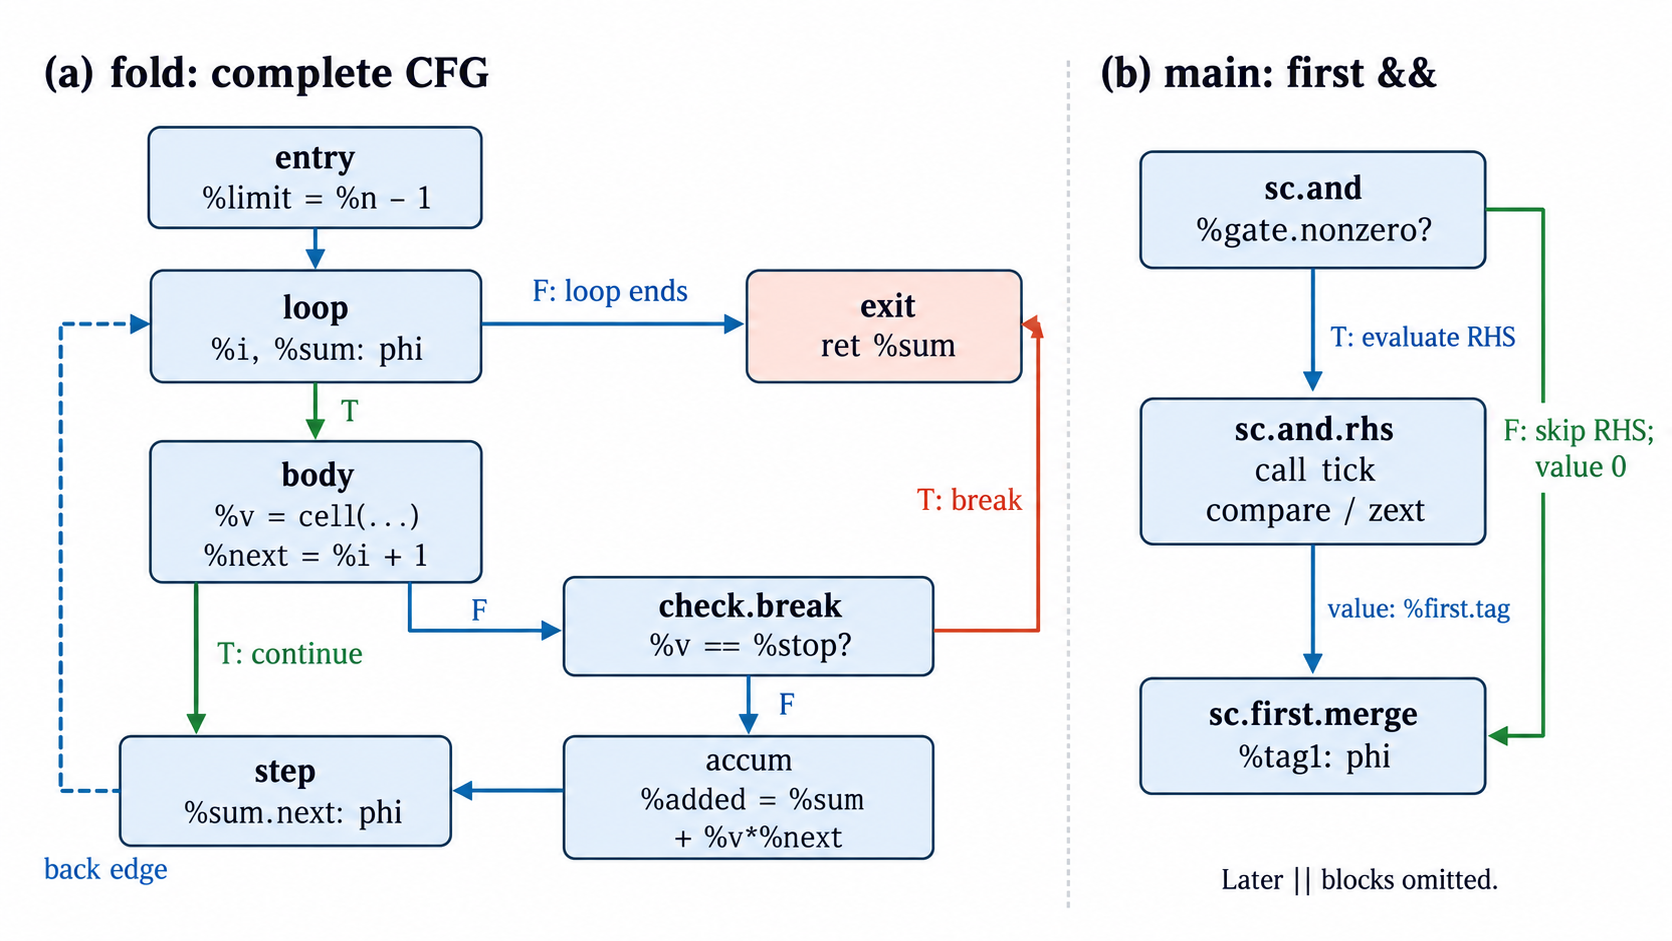
\includegraphics[width=\textwidth,keepaspectratio]{figures/fig3.png}
\caption{LLVM IR 控制流图。（a）\texttt{fold} 函数的完整 CFG，虚线表示循环回边；body 的 T/F 分别对应 \texttt{v==0} 的真假分支，continue 与 break 分别跳转至 \texttt{step} 和 \texttt{exit}。（b）\texttt{main} 中首个 \texttt{\&\&} 的短路求值子图，左操作数为假时跳过 \texttt{tick} 调用，为真时执行右操作数，并在 phi 节点合并结果。后续 \texttt{||} 相关基本块未展示。}
\label{fig:llvm-fold-cfg}
\end{figure}

\subsubsection{循环、break 与 continue}
\label{sec:sysy-ir-loops}
\texttt{while} 的循环条件位于 \texttt{loop}，循环体完成后经 \texttt{step} 回到条件块；索引已在 \texttt{body} 中、判断 \texttt{continue} 之前递增。\texttt{continue} 保留已有累计和并经 \texttt{step} 回跳，\texttt{break} 则直接到达退出块。表\ref{tab:source-cfg-ssa}按源语句对应其控制流边与 SSA 状态，说明每条跳转保留了哪一项源语义。

\begin{table}[H]
\centering\small
\caption{选取 \texttt{fold} 的关键源语句，逐项映射到 CFG 与 SSA}
\label{tab:source-cfg-ssa}
\begin{tabularx}{\textwidth}{L{4.45cm}L{3.0cm}Y}
\toprule\rowcolor{tableHead}SysY 源构造 & CFG 位置/边 & LLVM IR 状态 \\
\midrule
\texttt{int i=0,sum=0;} & \texttt{entry}$\to$\texttt{loop} & 两条 phi 的初次来值均为 0。\\
\texttt{while(i<=n-1)} & \texttt{loop} 条件及回边 & \texttt{icmp sle}；\texttt{\%i/\%sum} 为当前迭代状态。\\
\texttt{v=cell(...); i=i+1;} & \texttt{body} & 调用结果 \texttt{\%v}；递增值 \texttt{\%next}。\\
\texttt{if(v==0) continue;} & \texttt{body}$\to$\texttt{step} & 保留 \texttt{\%sum}，索引仍推进。\\
\texttt{if(v==stop) break;} & \makecell[l]{\texttt{check.break}\\$\to$\texttt{exit}} & 跳过累加与回边，返回当前 \texttt{\%sum}。\\
\texttt{sum=sum+v*i;} & \texttt{accum}$\to$\texttt{step} & 新值 \texttt{\%added} 进入 \texttt{\%sum.next}。\\
\texttt{return sum;} & \texttt{exit} & \texttt{ret i32 \%sum}，没有额外 exit phi。\\
\bottomrule
\end{tabularx}
\end{table}

\subsubsection{SSA 与 phi：变量赋值、前驱和支配关系}
\label{sec:sysy-ir-ssa}
源程序对 \texttt{i/sum} 的重复赋值，在 SSA 中分别产生新的值。循环入口与回边、正常累加与 continue 路径会带来不同值，phi 必须根据进入基本块的前驱边选择，才能实现对应的变量状态。

phi 的 incoming pair 是“值、前驱块”而非“条件、候选值”，其使用点视为对应入边\cite{llvm}。本例三个 phi 的关系如下：
\begin{enumerate}[itemsep=0.1em,topsep=0.1em]
\item \texttt{\%i = phi i32 [0,\%entry],[\%next,\%step]}：首次从 entry 取 0；以后从 step 取 body 已算好的 next。body 支配 step，故 continue 和累加两条到达 step 的路径都已定义 next。
\item \texttt{\%sum = phi i32 [0,\%entry],[\%sum.next,\%step]}：入口值为 0；每次回边取 step 内先行定义的 sum.next，而非不加区分地取 added。
\item \texttt{\%sum.next = phi i32 [\%sum,\%body],[\%added,\%accum]}：

body 入边是 continue，取旧 sum；accum 入边取刚定义的 added。added 无须支配整个 step，只需在 \texttt{accum}$\to$\texttt{step} 边上可用。
\end{enumerate}

dominator tree 显示 loop 支配 body 与 exit、body 支配 step。accum 不支配 step，其值在此合流，体现支配边界与 phi 放置的关系。源变量 sum 在 SSA 中对应 sum、added、sum.next 多个值。break 必须绕过 step：若错误地走 step 回边，就继续下一轮而没有终止。正常退出由 loop、break 退出由 check.break 到达 exit，两条路径上的 \texttt{\%sum} 均已定义，所以 exit 直接使用它：前者是全部已完成轮次之和，后者不含 stop 元素；$n=0$ 时就是入口 0。

\subsubsection{短路求值与副作用保持}
\label{sec:sysy-ir-short-circuit}
\texttt{\&\&} 与 \texttt{||} 的语义包含是否执行右操作数，不能只比较最终真假值。图\ref{fig:llvm-fold-cfg}右侧的子图用于解释 \texttt{gate != 0 \&\& tick(...)} 中调用的执行条件。

图中控制判断先决定是否进入 \texttt{sc.and.rhs}，tick 的全局写入只发生在真边上；假边直接进入 merge，并为 tag1 提供 0。若写成先 \texttt{call tick} 后 \texttt{select condition}，副作用在选择之前已经发生，select 只能选值，不能撤销写入。因此短路是执行路径的约束，不只是布尔值公式的等价；这里的先后关系是单线程语义顺序，不是硬件内存屏障。

手写 IR 中，上述判断位于 \texttt{sc.and}；真边进入 \texttt{sc.and.rhs} 执行调用，假边绕过调用，两条路径在 \texttt{sc.first.merge} 由 phi 合并 \texttt{tag1}。后续 \texttt{||} 及其右侧嵌套的 \texttt{\&\&} 同样通过条件分支控制调用是否发生，保留前述 \texttt{calls} 与 \texttt{tag} 的源语义。

\subsubsection{二维数组与 GEP 寻址}
\label{sec:sysy-ir-gep}
数组读写的等价性要求索引顺序、元素类型和行跨度一致；本例用 GEP 的类型结构表达二维数组的连续布局。

数组寻址也保留类型信息：main 的 \texttt{[2 x [3 x i32]]} GEP 先取对象层 0，再取行列；cell 接收 \texttt{[3 x i32]*}，行步长为 $3\times4=12$ 字节。\texttt{sext i32 to i64} 后形成 $\operatorname{base}+4(3r+c)$；行跨度由数组元素类型决定，与 8 字节指针宽度无关。此处二维数组的元素连续存储，其布局区别于指针数组。

\subsubsection{浮点运算与类型转换}
\label{sec:sysy-ir-float}
\texttt{float\_stats.ll} 使用 LLVM \texttt{float} 类型表达前述单精度计算，将浮点算术、整数循环条件与浮点筛选分别表示，保留源程序的运算顺序和转换位置。

\texttt{affine} 依次执行 \texttt{fmul float}、\texttt{sitofp i32 \%offset to float} 和 \texttt{fadd float}，对应先乘法、再将整数参数转换为浮点、最后相加。\texttt{sum\_positive} 的循环条件用 \texttt{icmp sge i32} 比较整数 \texttt{n} 与 \texttt{i+1}；\texttt{fcmp ogt float \%v,0.0} 则判断仿射结果是否为正，并以 \texttt{br} 选择累加或跳过。循环入口的 \texttt{phi i32/phi float} 保存索引与累计状态，\texttt{step} 中的 \texttt{phi float} 合并旧累计和与 \texttt{fadd} 产生的新值。

\texttt{main} 先用 \texttt{fadd} 加入 0.25，再以 \texttt{fptosi float \%result to i32} 表达向零截断；分母先由 \texttt{add i32} 计算 \texttt{n+1}，经 \texttt{sitofp} 转为 \texttt{float}，最后执行 \texttt{fdiv}。IR 未使用 \texttt{fast/contract} 标志，乘法与加法保持为分离操作，与式\eqref{eq:sysy-float-oracle}中的逐步舍入定义对应。转换与比较的等价性限定在前述有效输入域内，不据此扩展到越界转换或特殊浮点值。

\addtocontents{toc}{\protect\Needspace{4em}}
\subsection{RISC-V 汇编等价实现与底层机制}
\label{sec:sysy-riscv}
RISC-V 实现面向 RV64GC 指令集，用机器指令完成数值运算，用 branch/label 组织控制流，并按 LP64D ABI 传递参数、保存活跃值和返回结果。下面分别对应 SysY 的运算、控制和函数调用语义。

\subsubsection{整数运算与 RISC-V 指令映射}
\label{sec:sysy-riscv-integer}

RV64 的寄存器/地址为64位，但 SysY int 的存储和运算仍为32位。整数程序的 lw 读4字节再符号扩展，sw 只写低32位；addw、mulw 形成32位结果后符号扩展，divw/remw 对低32位做有符号除余。循环递减界限采用 \texttt{addiw ..., -1}\cite{riscv-isa}。替换成64位 long 运算会改变位宽截断约束；数组基址相加则使用完整64位 add，以保留地址位宽。实验输入已排除有符号溢出。

\subsubsection{条件分支与循环控制}
\label{sec:sysy-riscv-branches}
整数 \texttt{fold} 在 \texttt{.Lfold\_loop} 用 \texttt{bgt s3,s1,.Lfold\_exit} 判断循环结束；\texttt{call cell} 后先执行 \texttt{addiw s3,s3,1} 递增索引。随后 \texttt{beqz s5,.Lfold\_loop} 实现 continue，\texttt{beq s5,s2,.Lfold\_exit} 实现 break；其顺序保证 stop=0 时先跳过零元素。正常累加由 \texttt{mulw/addw} 完成，再用 \texttt{j .Lfold\_loop} 形成回边。

整数 \texttt{main} 的 \texttt{beqz s2,.Lsc\_or} 在 gate=0 时跳过第一个 \texttt{tick}；到达 \texttt{.Lsc\_or} 后，\texttt{beqz s2,.Lsc\_add2} 跳过 \texttt{||} 右侧。\texttt{bgez a0,.Lsc\_not} 决定嵌套 \texttt{\&\&} 是否调用 \texttt{tick}，\texttt{bnez s2,.Lcompute} 实现 \texttt{!gate} 的真假选择。浮点循环在 \texttt{.Lfloat\_loop} 用 \texttt{blt s1,t0,.Lfloat\_exit} 实现 \texttt{n>=i+1}；\texttt{flt.s} 的结果经 \texttt{beqz} 决定是否累加，随后在 \texttt{.Lfloat\_step} 递增索引并回跳。

\subsubsection{函数参数传递与调用约定}
\label{sec:sysy-riscv-parameters}
整数函数 \texttt{fold} 的数组地址、n 和 stop 分别放在 \texttt{a0/a1/a2}。\texttt{sum\_positive} 的数组地址和 n 使用 \texttt{a0/a1}，scale 作为第一个浮点参数使用 \texttt{fa0}；整数参数与浮点参数按各自的寄存器序列分配。

\texttt{float\_stats.S} 中 \texttt{affine} 是仅有乘法、转换、加法和 ret 的叶函数，没有栈帧。图\ref{fig:riscv-call-frame}将汇编指令与 LP64D 参数分配对照：x 与 scale 分别使用 \texttt{fa0/fa1}；整数和浮点参数寄存器独立分配，因此第三个源参数 offset 使用 a0，而不是 a2；float 返回复用 fa0\cite{riscvabi}。

\subsubsection{寄存器保存与函数调用}
\label{sec:sysy-riscv-save}
函数调用可能改写 caller-saved 寄存器，跨调用仍需使用的状态必须由调用方保护；使用 callee-saved 寄存器的函数则负责保存并恢复调用者的值。\texttt{sum\_positive} 调用 \texttt{affine}，可用于观察这两类责任。

在 \texttt{call affine} 前，后续仍需要数组地址、n、i、scale 与累计 sum，分别保留在 \texttt{s0/s1/s2/fs0/fs1}。当前元素 x 已装入 fa0，scale 从 fs0 复制到 fa1，i 从 s2 复制到 a0；返回后 fa0 改为仿射结果 v。计算元素地址的 t0 此时已无后续用途，而 affine 会改写 ft0。这些 caller-saved 临时寄存器的值不受被调用者保护，因此本实现将跨调用的活跃值保存在 callee-saved 寄存器中。

\subsubsection{栈帧组织与数据保护}
\label{sec:sysy-riscv-frame}
图\ref{fig:riscv-call-frame}对照叶函数的参数映射与非叶函数的保存区：\texttt{affine} 不建立栈帧，\texttt{sum\_positive} 使用 64 字节栈帧保存返回地址和寄存器。图中的偏移对应其入口保存和出口恢复指令。

以减去 64 后的新 \texttt{sp} 为基准，保存槽依次为 \texttt{fs1:16(sp)}、\texttt{fs0:24(sp)}、\texttt{s2:32(sp)}、\texttt{s1:40(sp)}、\texttt{s0:48(sp)} 和 \texttt{ra:56(sp)}；各槽占 8 字节，0--15 字节未使用。它们与 \texttt{float\_stats.S} 的保存、恢复指令逐项对应。

\begin{figure}[H]
\centering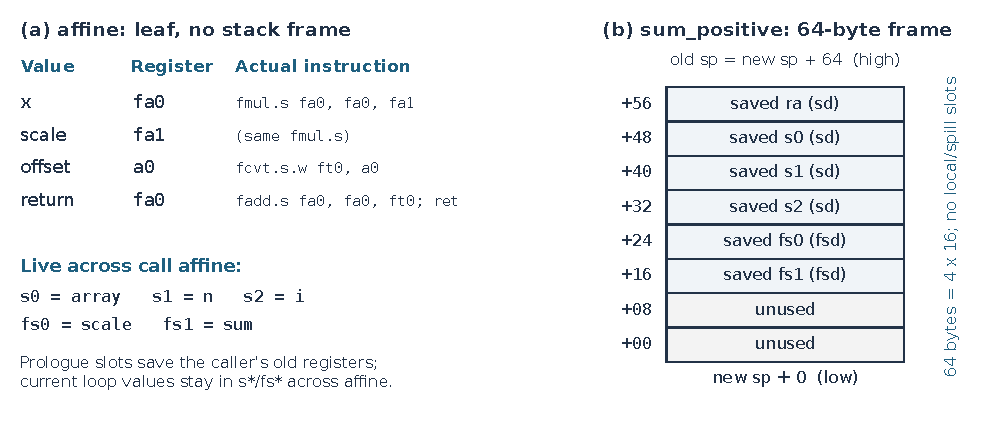
\includegraphics[width=\textwidth]{figures/riscv-call-frame.pdf}
\caption{左：\texttt{affine} 的参数映射，该叶函数不建立栈帧；右：\texttt{sum\_positive} 的非叶栈帧。偏移以减去 64 后的新 sp 为基准，每格 8 字节；0--15 字节未使用，没有局部数组或 spill 槽。}
\label{fig:riscv-call-frame}
\end{figure}

\Needspace{4\baselineskip}
要区分两种保护：当前循环状态跨 affine 调用留在 s/fs 寄存器中，该叶函数确实不修改它们；栈上保存的则是进入 sum\_positive 时\emph{调用者原来的} s/fs 值，并非每轮当前 sum 的副本。call 改写 ra，故入口将原返回地址存于 \texttt{56(sp)}。退出时先把当前 fs1 复制到 fa0，再依次恢复 fs1/fs0/s2/s1/s0/ra，最后加回 64 并 ret。$64=4\times16$ 保持栈对齐，fsd/fld 保存完整64位寄存器状态。

\subsubsection{浮点运算与类型转换}
\label{sec:sysy-riscv-float}
浮点等价实现需要保持单精度运算的舍入位置，并使浮点到整数的转换采用 SysY 所要求的向零截断。

浮点乘加使用 \texttt{fmul.s/fadd.s} 两次舍入，无融合乘加；整数 offset 用 \texttt{fcvt.s.w}，最终 \texttt{fcvt.w.s ...,rtz} 与 IR 的 \texttt{fptosi} 对应向零截断。这里保留的是\hyperref[sec:sysy-float-semantics]{浮点示例计算定义}中的各个舍入位置：\texttt{affine} 不使用 \texttt{fmadd.s}，正值累计和结果偏置分别使用独立的 \texttt{fadd.s}；分母经 \texttt{addiw} 和 \texttt{fcvt.s.w} 后，\texttt{fdiv.s} 产生最后一项输出。数组元素通过 \texttt{flw/fsw} 按 4 字节访问，与保存浮点寄存器状态的 \texttt{fsd/fld} 用途不同。源程序计算过程、有效域与 oracle 已在示例设计部分定义，这里据此核对机器指令的位宽、转换模式和运算顺序。

\subsubsection{LLVM IR 与 RISC-V 的语义映射对照}
\label{sec:sysy-semantic-mapping}
表\ref{tab:sysy-semantic-mapping}归纳两种手写实现对同一 SysY 语义的表达。各项机制均对应当前 \texttt{control\_matrix} 或 \texttt{float\_stats} 的手写 IR 与汇编文件中的实际操作。

\begingroup
\small
\setlength{\tabcolsep}{4pt}
\begin{longtable}{L{2.0cm}L{4.0cm}L{4.0cm}L{4.5cm}}
\caption{SysY 语言特性在 LLVM IR 与 RISC-V 汇编中的实现对应关系}
\label{tab:sysy-semantic-mapping}\\
\toprule\rowcolor{tableHead}SysY 语义 & LLVM IR 关键机制 & RISC-V 关键机制 & 语义保持要点 \\
\midrule
\endfirsthead
\toprule\rowcolor{tableHead}SysY 语义 & LLVM IR 关键机制 & RISC-V 关键机制 & 语义保持要点 \\
\midrule
\endhead
\bottomrule
\endfoot
整数运算 & \texttt{add/mul i32}、\texttt{sdiv/srem} & \texttt{addw/mulw}、\texttt{divw/remw} & 保持 32 位整数结果及有符号除余行为。\\
条件分支 & 整数 \texttt{icmp/br}；浮点 \texttt{fcmp ogt/br} & \texttt{bgt/beqz/beq} 等分支；\texttt{flt.s} 后分支 & 比较对象、真假方向及执行路径一致。\\
循环 & \texttt{loop/body/step/exit} 基本块与回边 & 循环标签、\texttt{addiw} 与 \texttt{j} 回跳 & 保持迭代边界、索引递增及提前终止。\\
变量更新 & \texttt{phi} 合并 SSA 值；\texttt{load/add/store} 更新全局状态 & 寄存器更新；\texttt{lw/addiw/sw} 更新 \texttt{calls} & 按实际前驱路径选择状态并保留可观察写入。\\
短路求值 & 条件 \texttt{br} 决定 \texttt{call tick} 是否执行，phi 合流 & \texttt{beqz/bgez} 等跳转绕过或进入调用 & RHS 的全局副作用仅在源语义要求的路径发生。\\
数组访问 & 类型化 \texttt{getelementptr}，元素 \texttt{load/store} & 行列偏移、\texttt{slli/add}，整数 \texttt{lw/sw}、浮点 \texttt{flw/fsw} & 二维行跨度 12 字节，整数和浮点元素均占 4 字节。\\
函数调用 & 带类型的 \texttt{call/ret} 及参数、返回值 & LP64D 的 \texttt{a/fa} 参数与返回寄存器，\texttt{call/ret} 及保存恢复 & 参数类别、顺序、返回值和跨调用活跃状态一致。\\
浮点运算 & \texttt{float} 上的 \texttt{fmul/fadd/fdiv} & \texttt{fmul.s/fadd.s}、\texttt{fdiv.s} & 保持 binary32 运算顺序和分离乘加的舍入位置。\\
类型转换 & \texttt{sitofp} 与 \texttt{fptosi} & \texttt{fcvt.s.w} 与 \texttt{fcvt.w.s ...,rtz} & 整数到单精度转换；浮点到整数向零截断。\\
\end{longtable}
\endgroup

同一 SysY 语义在 LLVM IR 中主要通过类型化操作、控制流和 SSA 表达，在 RISC-V 中则由机器指令、寄存器状态及 ABI 约束共同实现。表中的对应关系属于语义层面的归纳，并非指令严格一一对应；循环、短路与函数调用通常需要多个基本块或多条机器指令协作。下面将两种独立实现与源程序基准统一接入运行库，再分别构建并验证。

\subsection{SysY 运行时库的构建与集成}
\label{sec:sysy-runtime}
输入输出函数由链接的 SysY 运行库提供；程序只调用相应接口，目标 glibc 承担底层输入输出。运行库编译为目标对象并归档为 \texttt{libsylib.a}，再参与各程序的最终静态链接。
实验参考 SysY2022 语言定义与运行库说明\cite{sysyspec}。由于课程专用运行库原件未提供，本实验采用公开的 SysY2022 兼容实现\cite{runtime}；\texttt{getint/getfloat/putint/putfloat/putch} 由该运行库提供，并调用目标 glibc。

运行库的构建命令如下，目标架构与三个程序路径均为 RV64GC/LP64D：
\begin{lstlisting}[caption={SysY 运行库对象与静态归档的构建},label={lst:sysy-runtime-build}]
riscv64-linux-gnu-gcc -std=c11 -O2 -fcommon -march=rv64gc -mabi=lp64d -c runtime/sylib.c -o artifacts/sysy/objects/sylib.o
riscv64-linux-gnu-ar rcs artifacts/sysy/objects/libsylib.a artifacts/sysy/objects/sylib.o
\end{lstlisting}
运行库头文件含全局暂定定义，使用 \texttt{-fcommon} 兼容其定义方式。链接 map 显示 \texttt{sylib.o} 满足 getint 等引用。运行库 stderr 的 \texttt{TOTAL: 0H-0M-0S-0us} 表示未启用计时接口时的累计时间，不用于性能分析。

\subsection{三种程序实现的编译与链接}
\label{sec:sysy-build}
本节将源程序基准、手写 LLVM IR 和手写 RISC-V 汇编分别编译为目标对象，并链接为独立的 RISC-V ELF 程序。源实现由 Clang 以 \texttt{-x c} 按 C 兼容子集处理 \texttt{.sy} 文件，通过 \texttt{-include runtime/sylib.h} 注入运行库声明；这一构建基准不等同于自行实现完整 SysY 编译器。LLVM 14 有类型指针 IR 与 RV64GC/LP64D 汇编分别构建。自动生成的 IR 与汇编仅用于结果对照。手写 IR 经验证后由 llc 生成目标文件，手写汇编独立汇编，二者均按 SysY 源语义编写，互不作为对方的自动生成结果。两个示例的六个程序均静态链接 \texttt{libsylib.a} 和目标 glibc，以 \texttt{qemu-riscv64} 执行。目标对象的 ELF 记录显示 RISC-V、RVC、double-float ABI 标志。

图\ref{fig:sysy-build-paths}显示源程序、手写 IR 与手写汇编三条构建路径。由 SysY 到手写 IR/汇编的虚线表示按源语义编写等价实现；后续实线表示工具处理。每条路径分别链接生成一个 ELF 程序，再使用相同输入比较输出。
\begin{figure}[H]
\centering
\begin{tikzpicture}[
  sysybox/.style={draw=blueGray,rounded corners=2pt,fill=softBlue,align=center,text width=3.85cm,minimum height=1.08cm,font=\small},
  sysywide/.style={sysybox,text width=6.6cm},
  buildarrow/.style={-{Stealth[length=2mm]},thick,draw=blueGray},
  writearrow/.style={buildarrow,dashed}
]
\node[sysywide] (meaning) at (0,0) {SysY 示例程序与语义};
\node[sysybox] (source) at (-4.7,-1.75) {SysY 源实现 \texttt{.sy}\\Clang 14 交叉编译};
\node[sysybox] (ir) at (0,-1.75) {手写 LLVM IR \texttt{.ll}\\\texttt{llvm-as / opt / llc}};
\node[sysybox] (asm) at (4.7,-1.75) {手写 RISC-V \texttt{.S}\\交叉 GCC 调用汇编器};
\node[sysybox] (so) at (-4.7,-3.35) {\texttt{source.o}};
\node[sysybox] (io) at (0,-3.35) {\texttt{llvm.o}};
\node[sysybox] (ao) at (4.7,-3.35) {\texttt{asm.o}};
\node[sysywide] (link) at (0,-5.05) {各路径分别静态链接\\\texttt{libsylib.a + glibc}};
\node[sysywide] (elf) at (0,-6.55) {三种 RISC-V ELF 程序};
\node[sysywide] (qemu) at (0,-8.05) {\texttt{qemu-riscv64}：相同输入与输出比较};
\draw[buildarrow] (meaning.south west) -- (source.north);
\draw[writearrow] (meaning.south) -- (ir.north);
\draw[writearrow] (meaning.south east) -- (asm.north);
\draw[buildarrow] (source) -- (so);
\draw[buildarrow] (ir) -- (io);
\draw[buildarrow] (asm) -- (ao);
\draw[buildarrow] (so.south) -- (link.north west);
\draw[buildarrow] (io.south) -- (link.north);
\draw[buildarrow] (ao.south) -- (link.north east);
\draw[buildarrow] (link) -- (elf);
\draw[buildarrow] (elf) -- (qemu);
\end{tikzpicture}
\caption{SysY、手写 LLVM IR 与手写 RISC-V 汇编的三条构建路径。虚线表示按语义手写，实线表示构建与执行；三种实现分别生成可执行程序。}
\label{fig:sysy-build-paths}
\end{figure}

以下以 \texttt{control\_matrix} 为例列出构建命令；\texttt{float\_stats} 使用同一脚本和选项，仅替换程序名。
\begin{lstlisting}[caption={源程序、手写 IR 与手写汇编分别生成目标文件},label={lst:sysy-object-build}]
clang-14 --target=riscv64-linux-gnu --gcc-toolchain=/usr -march=rv64gc -mabi=lp64d -std=c11 -fcommon -ffp-contract=off -O0 -x c -include runtime/sylib.h -c src/sysy/control_matrix.sy -o artifacts/sysy/objects/control_matrix.source.o
llvm-as-14 src/llvm/control_matrix.ll -o artifacts/sysy/objects/control_matrix.bc
opt-14 -verify -disable-output artifacts/sysy/objects/control_matrix.bc
llc-14 -O0 -mtriple=riscv64-linux-gnu -mattr=+m,+a,+f,+d,+c -target-abi=lp64d -filetype=obj artifacts/sysy/objects/control_matrix.bc -o artifacts/sysy/objects/control_matrix.llvm.o
riscv64-linux-gnu-gcc -march=rv64gc -mabi=lp64d -c src/riscv/control_matrix.S -o artifacts/sysy/objects/control_matrix.asm.o
\end{lstlisting}
\texttt{llvm-as-14} 将 IR 文本解析为 bitcode，\texttt{opt-14 -verify} 检查结构合法性，\texttt{llc-14 -filetype=obj} 直接生成目标对象。\texttt{riscv64-linux-gnu-gcc -c} 对 \texttt{.S} 文件调用汇编器，保留独立手写汇编路径。源程序的 \texttt{-ffp-contract=off} 关闭乘加融合，与手写 IR 和汇编的分离乘加一致。

\noindent\begin{minipage}{\linewidth}
下列命令链接 IR 路径；源实现和汇编实现分别替换为 \texttt{source.o} 与 \texttt{asm.o}。运行时由测试程序将输入送入标准输入，并比较标准输出与退出状态。
\begin{lstlisting}[caption={IR 路径的静态链接与执行工具},label={lst:sysy-link-run}]
riscv64-linux-gnu-gcc -static -no-pie -march=rv64gc -mabi=lp64d artifacts/sysy/objects/control_matrix.llvm.o artifacts/sysy/objects/libsylib.a -Wl,-Map,artifacts/sysy/control_matrix.llvm.map -o artifacts/sysy/bin/control_matrix.llvm
qemu-riscv64 artifacts/sysy/bin/control_matrix.llvm
\end{lstlisting}
\end{minipage}

三条路径分别生成可执行程序后，还需在相同输入下与独立预期逐一比较。仅让三份程序相互比较无法排除共同实现错误，因而下面同时检验输出、退出状态和针对特定语义风险的负对照。

\subsection{运行结果与语义一致性验证}
\label{sec:sysy-results}
本节依据两个示例的源语义检验三种独立实现，依次说明测试设计、实际运行结果、注错负对照和验证范围，以区分结构合法、正常退出与语义正确这几种不同条件。

\subsubsection{测试用例与独立预期}
\label{sec:sysy-test-design}
三种实现使用同一组测试输入，并分别与独立数学 oracle 的预期输出比较，同时检查程序退出状态。整数用例限定在前述有效域，排除数组越界、整数溢出和除零；浮点 oracle 按 binary32 逐步舍入，结果按正文给出的绝对/相对组合容差判断，整数输出精确比较。

整数测试包括 20 个固定用例与 80 个按固定种子生成的用例，覆盖空循环、不同停止位置、零值跳过、短路分支、正负除余与增量边界。浮点测试包括 10 个固定用例与 50 个生成用例，覆盖空输入、零或负 scale、正负值筛选、非整数结果与输入边界。生成器先将浮点输入舍入为 binary32，再以十六进制浮点形式送入运行库，减少十进制文本转换歧义。

预期输出独立于三种实现计算：整数采用前述加权前缀和与显式符号除余定义，浮点采用式\eqref{eq:sysy-float-oracle}的逐步舍入过程，再计算偏置、截断与归一化结果；五个手算锚点用于核对 oracle 本身。每次执行保存输入、预期、标准输出、标准错误和退出码，只有退出 0 且输出满足判据才计为通过。浮点输出按数值解析比较，而非字符串逐字比较；容差适用于两个浮点输出，中间的整数输出仍要求精确相同。

\subsubsection{三种实现的运行结果}
\label{sec:sysy-run-results}
100 个整数和 60 个浮点用例在三种实现上共运行 480 次，\textbf{480/480 次通过}，失败0，均退出0；随机种子为 \texttt{24115602412565}。180次浮点结果与 binary32 oracle 数值精确一致。完整初值例的加权和 $1+4-12+20+30=43$，加偏置后53；第四位置 $-3$ 触发 break 时仅累加 $1+4$，得到15。手算结果作为独立参考值，用于验证三种实现的输出。

$n=1,scale=1,a=[0.5]$ 的输出是 \texttt{0x1.8p-1 0 0x1.8p-2}，即0.75、0、0.375；$n=3,scale=0.1,a=[0.1,0.2,0.3]$ 对应的 binary32 结果为3.309999942779541，打印为 \texttt{0x1.a7ae14p+1}，相对于精确实数3.31存在舍入误差。180 次数值精确一致是当前用例的实际观察；测试仍使用既定容差判据，不由这一观察推断所有输入均严格相等。

\subsubsection{错误注入与测试有效性分析}
\label{sec:sysy-mutation-analysis}

为检查测试集对特定语义错误的辨识力，表\ref{tab:cases}列出用例、注错方式及输出差异。

\begin{table}[H]
\centering\small
\caption{测试用例与注错变体的检出结果}
\label{tab:cases}
\begin{tabularx}{\textwidth}{L{2.05cm}L{3.75cm}L{3.7cm}Y}
\toprule\rowcolor{tableHead}语义风险 & 用例设计 & 注错变体/输出差异 & 检出结论 \\
\midrule
短路副作用 & gate=0，tick 修改 calls & 删首个短路跳转；calls 从应有0变1，tag 从6变7 & 已检出；退出0仍错误。\\
有符号余数 & 被除数 $-5$、除数3；应为商$-1$、余$-2$ & \texttt{remw}$\to$\texttt{divw}；余数输出$-1$ & 已检出；区分商与余。\\
浮点转整数 & 仿射结果加偏置得到0.75 & \texttt{rtz}$\to$\texttt{rne}；整数从应有0变1 & 已检出；浮点输出仍正确。\\
二维数组寻址 & 六个位置、不同增量及位置权重 & 数组用例均通过；未构造错误行跨度变体 & \textbf{未测试错误行跨度的检出能力}。\\
\bottomrule
\end{tabularx}
\end{table}

另外构造 3 个注错变体，\textbf{3/3 均被测试集检出}；这些负对照不计入480次正常程序测试。三个变体分别改变右侧调用是否执行、余数运算及浮点到整数的舍入模式。它们均正常退出，但 \texttt{calls/tag}、负数余数或整数转换值偏离独立预期，说明退出成功本身不足以判定语义正确。该结果仅表明当前用例能够辨识这三种实际注入的错误；二维数组用例虽然全部通过，尚未实施错误行跨度变体，不能将其写成已经验证的检出能力。

\subsubsection{语义验证的适用范围与局限}
\label{sec:sysy-validation-limits}
测试覆盖上述有效域中的有限样本，未进行全输入空间的形式化等价证明。整数有效域排除数组越界、有符号溢出、除零及 \texttt{INT\_MIN/-1}；浮点验证不扩展到 NaN/Inf、次正规数或越界转换，也不包含未声明支持的输入情况。因此，480 次执行通过支持的是指定样本和判据下的功能与输出一致性。

这里的 \texttt{qemu-riscv64} 用户态模拟用于检查 RISC-V 指令在 Linux ABI 下的功能行为，不构成真实 RISC-V 硬件上的性能测量\cite{qemu}。

